\documentclass[11pt, oneside]{article}
\usepackage{titling, hyperref, geometry, amsmath, amssymb, algorithm, graphicx, textcomp, subcaption, cancel}
\usepackage[noend]{algpseudocode}
\usepackage[cache=false]{minted}
\geometry{a4paper}

\hypersetup{
  colorlinks=true,
  urlcolor=cyan
}

\newcommand{\emphasis}[1]{\textcolor{blue}{\textbf{\textit{#1}}}}
\graphicspath{{./images/}}

\title{Range Minimum Query with Fischer-Heun}
\author{Stephen Huan\\ Edited by: Udbhav Muthakana}
\date{April 5, 2020}

\begin{document}
\maketitle

\section{Definition}

The \emphasis{Range Minimum Query} (RMQ) problem is defined as follows: \\
Given an array \( A \) with length \( n \) and two indexes \( i, j \mid i \leq j \),
find the smallest element between \( i \) and \( j \) (inclusive on both ends).

First, we should return the index \( k \) of the smallest element.
Note that given \( k \) we can access the value
with \( A[k] \), but the reverse is not true - in an array with identical values,
it's impossible to determine which index the value came from.

The notation I will use for running time is \( \langle f, g \rangle \),
where \( f \) is the preprocessing time and \( g \) is the query time. For example,
the naïve algorithm of scanning every element between \( i \) and \( j \)
is \( \langle O(1), O(n) \rangle \), as it has no preprocessing time
but could scan the entire array for every query in the worst case.

\section{Algorithms}
\subsection{Fenwick Trees and Segment Trees}

Two classic data structures for this problem are Fenwick trees (more commonly known as Binary Indexed Trees, or ``BITs'')
and segment trees. BITs can solve RMQ in \( \langle O(n \log n), O(\log n) \rangle \), while segment trees
can do it in \( \langle O(n), O(\log n) \rangle \). Both also support a wide variety of functions (sum, XOR, etc.) and
allow dynamic updates of single values and ranges. If you are interested in the aforementioned data structures for competitive programming,
read the SCT lectures linked in the appendix. Although this lecture's algorithm is more limited in its functions
and cannot update, it has asymptotically optimal construction and query times - \( \langle O(n), O(1) \rangle \)!

\subsection{Dynamic Programming}

There are only \( \Theta(n^2) \) possible queries because \( i \) can take on \( n \) possible values
and \( j \geq i \) (there are exactly \( n + (n - 1) + (n - 2) + \ldots + 1 = \frac{n(n + 1)}{2} \) queries).

If we precompute every possible query, then we can answer them in \( O(1) \). Naïvely computing the table
with an \( O(n) \) scan for each query will take \( O(n^3) \) for all the queries.
Instead, we can use dynamic programming. Consider the base case of \( i = j \);
the minimum is the only element in the range. Now consider a range of length \( l \) starting
at \( i \), given the minima for all ranges of length \( l - 1 \).
The answer would just be the minimum between the range starting at \( i \) with a length of \( l - 1 \),
and the range starting at \( i + 1 \) with the same length. Although there is significant overlap between
the two ranges, this is fine because the minimum of two intersecting ranges is the minimum of the union
of the regions. Note that this is not true for addition - it would overcount the intersection.

\begin{figure}[h!]
\centering
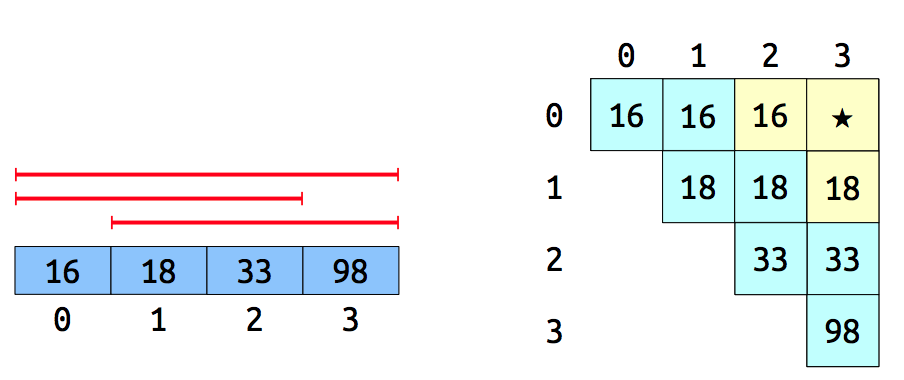
\includegraphics[scale=0.25]{dp}
\caption{Decomposing a range into smaller ranges and the DP table.}
\end{figure}

Since there are \( O(n^2) \) states and transitions between states are calculated in \( O(1) \),
this is an \( O(n^2) \) DP, yielding an \( \langle O(n^2), O(1) \rangle \) RMQ structure. We now have two solutions:
\( \langle O(1), O(n) \rangle \) with no preprocessing and \( \langle O(n^2), O(1) \rangle \) with full preprocessing. Can we get something in between?

\subsection{Sparse Tables}

Instead of precomputing all \( O(n^2) \) possible ranges, it suffices to only compute a certain subset of ranges
and still maintain constant time query. The key observation is that any range can be broken down into subranges
with lengths that are powers of two.

\begin{figure}[h!]
\centering
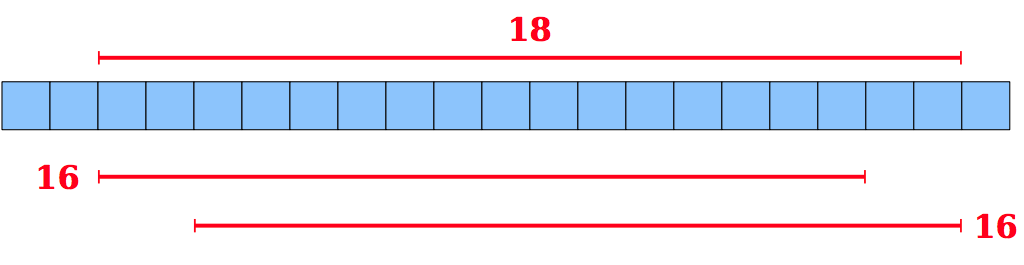
\includegraphics[scale=0.25]{sparse_decomp}
\caption{Breaking up a range into powers of two}
\end{figure}

For each starting index \( i \), precompute the minimum in the ranges with lengths
\( 1, 2, 4, \dots 2^l \), where \( l \) is at most \( \log n \). In order to answer a query,
find the largest \( k \) such that \( 2^k \leq j - i + 1 \). This is equivalent to finding the
most significant bit of \( j - i + 1 \), which can be done in constant time (if you are interested,
a lecture is given \href{http://web.stanford.edu/class/cs166/lectures/16/Slides16.pdf}{here}).
The simplest method is to compute \( \lfloor \log_2{(j - i + 1)} \rfloor \), but that can be slow.
\\
Then, think of the range \( [i, j] \) as the union between the ranges \( [i, i + 2^k] \) and \( [j - 2^k, j] \).
Each range has already been precomputed, so the query is \( O(1) \).

In order to precompute the \( O(n \log n) \) ranges, we use dynamic programming again.
The logic is identical to the \( 2^n \) jump pointers for the lowest common ancestor problem.
The base case of \( i = j \) is again to choose the only element in the range. Consider a range of length \( l \) starting
at \( i \), given the minima for all ranges of length \( \frac{l}{2} \). The answer would just be
the range starting at \( i \) with length \( \frac{l}{2} \) and the range starting at \( i + \frac{l}{2} \)
with the same length (the intuition is that \( 2^x \) is, by definition, \( 2 \cdot 2^{x - 1} \) so we can compute the answer to \( x \)
by combining two answers of \( x - 1 \)).

Overall, \emphasis{sparse tables} yield an \( \langle O(n \log n), O(1) \rangle \) solution to RMQ.
Can we get something else in between full preprocessing and no preprocessing?

\subsection{Block Decomposition}

Consider splitting the array into \( \frac{n}{b} \) blocks, where each block
has a size of \( b \). Compute the minimum value in each block.

\begin{figure}[h!]
\centering
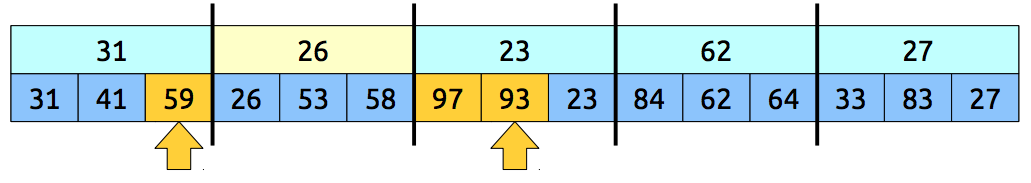
\includegraphics[scale=0.25]{block}
\caption{Array with block size \( b = 3 \)}
\end{figure}

Suppose \( i \) and \( j \) are in different blocks with blocks in between them
(the cases where \( i \) and \( j \) are in the same block, or they are in different but adjacent blocks
are trivial). To answer a RMQ query, scan from \( i \)'s position to the end of its block,
\( j \)'s position to the beginning of its block, and instead of scanning each element in between
\( i \) and \( j \), use the precomputed block minima.

The preprocessing time is \( O(b) \) to find the minimum in each block, times
\( \frac{n}{b} \) blocks for \( O(n) \). The query time is
\begin{itemize}
  \item \( O(1) \) to find the position of \( i \) and \( j \) in their blocks (divide by \( b \))
  \item \( O(b) \) to scan \( i \) and \( j \)'s blocks
  \item \( O(\frac{n}{b}) \) to scan block minima between \( i \) and \( j \).
\end{itemize}
The total query cost is \( O(b + \frac{n}{b}) \). How do we pick \( b \) to minimize this cost? Calculus.
\[ \frac{\mathrm{ d}}{\mathrm{ d}b} (b + n b^{-1}) = 1 - n b^{-2} = 0 \]
\[ 1 = n b^{-2} \]
\[ b^2 = n \]
\[ b = \sqrt{n} \]

We now have an \( \langle O(n), O(\sqrt{n}) \rangle \) solution to RMQ. This technique is
actually called ``Square root bucketing'' and has been covered in past SCT lectures.

\subsection{Hybrids}

Instead of naïvely scanning inside blocks and over the block minima, we can build another RMQ
structure on top! The algorithm is then as follows:
\begin{itemize}
  \item Split the input array into blocks of size \( b \).
  \item Form a smaller array of block minima.
  \item Create a ``summary'' RMQ structure over the block minima array.
  \item Create ``block'' RMQ structures for each block.
  \item Merge the results together for queries.
\end{itemize}

\begin{figure}[h!]
\centering
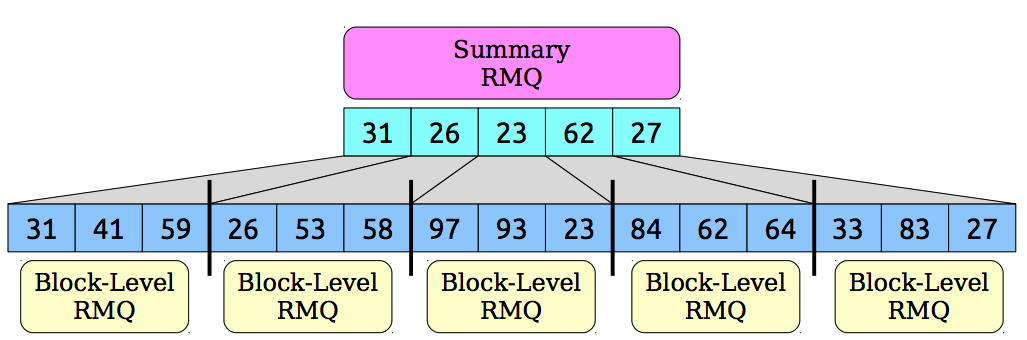
\includegraphics[scale=0.25]{summary}
\caption{Top level view of the overall RMQ structure}
\end{figure}

In order to analyze the running time of this new hybrid structure, let
\( \langle f(n), g(n) \rangle \) be the time for the block minima and
\( \langle p(n), q(n) \rangle \) be the time for each block.

The preprocessing time is then:
\begin{itemize}
  \item \( O(n) \) to compute the minimum for each block
  \item \( O(f(\frac{n}{b})) \) to construct the RMQ structure on the block minima
  \item \( O(\frac{n}{b} p(b)) \) to construct the RMQ structure for each block
\end{itemize}
resulting in a construction time of \( O(n + f(\frac{n}{b}) + \frac{n}{b} p(b)) \).

The query time is then:
\begin{itemize}
  \item \( O(g(\frac{n}{b})) \) to query the block minima
  \item \( O(q(b)) \) to query a block
\end{itemize}
resulting in a query time of \( O(g(\frac{n}{b}) + q(b)) \).

\subsubsection{Hybrid Example}

Suppose we use the \( \langle O(n \log n), O(1) \rangle \) sparse table
structure for both the top and bottom.
The preprocessing time is:
\[ O(n + f(\frac{n}{b}) + \frac{n}{b} p(b)) \]
\[ = O(n + \frac{n}{b} \log \frac{n}{b} + \frac{n}{b} b \log b) = O(n + \frac{n}{b} \log n + n \log b) \]
Suppose we pick \( b = \log n \).
\[ = O(n + \frac{n}{\log n} \log n + n \log {\log n}) \]
\[ = O(n \log {\log n}) \]

The query time is \( O(g(\frac{n}{b}) + q(b)) \), which
must be \( O(1) \) since both sparse tables have a query of \( O(1) \).

Wait a second. If we used hybridization to get an \( \langle O(n \log \log n), O(1) \rangle \) structure
from an \( \langle O(n \log n), O(1) \rangle \) structure, why can't we do it again?

\[ O(n + f(\frac{n}{b}) + \frac{n}{b} p(b)) = O(n + \frac{n}{b} \log \log n + n \log \log b) \]
Now pick \( b = \log \log n \)
\[ = O(n + n + n \log \log \log \log n) \]

Before we recur yet again, realize that there's a limit to this recursion. You can't have a block size of
less than 1, so we can't add an unlimited number of logarithms.

Let \( \log^{(i)} x \) denote appying the log function iteratively, e.g. \( \log^{(3)} x = \log \log \log x \). We define \( \log^* x = \min\{ i \geq 0 \mid \log^{(i)} x \leq 1\} \), i.e. the largest \( i \) such that after repeatedly applying log that many times the result is \( \geq 1 \). Some examples:
\begin{align*}
        \log^* 2 = 1 \\
        \log^* 4 = 2 \\
       \log^* 16 = 3 \\
    \log^* 65536 = 4 \\
\log^* 2^{65536} = 5 \\
\end{align*}
Since \( 2^{65536} \) is a gigantic number, \( \log^* x \) is probably never greater than 5.
Thus, we now have a beautifully recursive \( \langle O(n \log^* n), O(1) \rangle \) structure which is for all practical purposes \( \langle O(n), O(1) \rangle \).
This follows the same reasoning as the inverse Ackermann function - \textit{technically}
union-find is \( O(\alpha(m)) \), but we usually treat it as a constant.

However, union-find is asymptotically optimal i.e there does not exist a constant time
union-find structure. Does there exist an actual \( \langle O(n), O(1) \rangle \) structure?

\subsection{Fischer-Heun}

\subsubsection{Block Types}
Suppose we have the arrays \( B_1 = [1, 3, 2, 4] \) and \( B_2 = [10, 30, 20, 40] \).
Although the arrays are different, the answer to any RMQ query is going to be the same,
since they have a similar \emphasis{type} (which we'll represent as \( B_1 \sim B_2 \)).
If we find that two blocks have the same type, we can reuse the RMQ structure of one
for the other without computing it again. We'll also use the aforementioned sparse table
for the top and the fully precomputed solution for the blocks.
The precomputation time is then
\[ O(n + \frac{n}{b} \log n + (\text{\# of distinct blocks}) b^2) \]

We now have two questions:
\begin{enumerate}
  \item How do we tell if \( B_1 \sim B_2 \)?
  \item How many different types are there?
\end{enumerate}

\subsubsection{Detecting Block Types}
Intuitively, we might use the ``permutation type'', or element ordering.
If we sort the array and assign an id of 0 to the smallest element, 1 to the next, etc.
then the resulting order of ids is the permutation type. Going back to the previous example,
\( B_1 \) would have a permutation type of 0, 2, 1, 3, as would \( B_2 \).
If \( B_1 \) has the same permutation type as \( B_2 \), then \( B_1 \sim B_2 \).
However, the converse is not true. Consider \( B_1 = [4, 5, 1, 3, 2] \) and \( B_2 = [3, 4, 1, 5, 2] \).
The permutation type of \( B_1 \) is 3, 4, 0, 2, 1 while the permutation type of \( B_2 \) is 2, 3, 0, 4, 1
which are different.

However, \( B_1 \sim B_2 \) (this is not obvious, but brute force every possible range).
The fact that permutation type doesn't cover all the possibilities of two blocks being similar is fine
from a correctness standpoint. However, the number of possible permutations is \( b! \),
so \( b \) will have to be very small for the number of distinct blocks to be reasonable.
Intuitively, this is because permutation doesn't cover enough ``cases'' - the more cases
an approach covers, the less work the algorithm will have to do.

We now have a incorrect but fast solution. Observe that \( B_1 \) and \( B_2 \) will obviously
have the same answers for ranges of length 1. Because the pairwise relations are the same (in \( B_1 \) \( 4 < 5, 5 > 1, 1 < 3 \), etc.
while in \( B_2 \) \(3 < 4, 4 > 1, 1 < 5 \)), they will have the same answers for ranges of length 2.
By the same inductive argument the dynamic programming relied on earlier, they must have the same answers for every range.
To see why this is not true, consider three numbers, \( a, b, c \). If the pairwise relations are the same,
then we know the relationship between \( a, b \) and \( b, c \). Can we find the minimum element from this?

\newpage

\begin{table}[ht!]
\centering
\begin{tabular}{ cccc }
 \( a, b \) & \( b, c \) & \( a, c \) & minimum \\
 \hline
 \( < \) & \( < \) & \( < \) & \( a \) \\
 \( > \) & \( < \) & \( ? \) & \( b \) \\
 \( < \) & \( > \) & \( ? \) & \( ? \) \\
 \( > \) & \( > \) & \( > \) & \( c \) \\
 \hline
\end{tabular}
\caption{Binary relations table}
\end{table}

Note that in the case of \( a > b \) and \( b < c \), it's unknown whether \( a > c \),
but it's irrelevant because \( b \) must be the minimum. However, in the case of \( a < b \)
and \( b > c \), it's actually impossible to determine the minimum. Take the example of
\( B_1 = [5, 10, 1] \) and \( B_2 = [5, 10, 7] \). In both cases, the pairwise relations are the same.
However, \( B_1 \cancel{\sim} B_2 \) because the minimum element is at index 2 for \( B_1 \) and
at index 0 for \( B_2 \). Although the number of possible pairwise relations is \( 2^b \), which is reasonable
for \( b = \log n \), this approach will not yield correct answers.

We've seen how permutations have too many possibilities but are correct, while binary relations have
few possibilities and are incorrect. Is there something in between?

The next approach stems from the observation that if \( B_1 \sim B_2 \), they must have minimum elements
at the same position. If they didn't, a range query over the length of the array would yield different answers.
This property must also hold recusively on the subarrays to the left and to the right of the minimum.
These observations lead us to Cartesian trees.

\begin{figure}[h!]
\centering
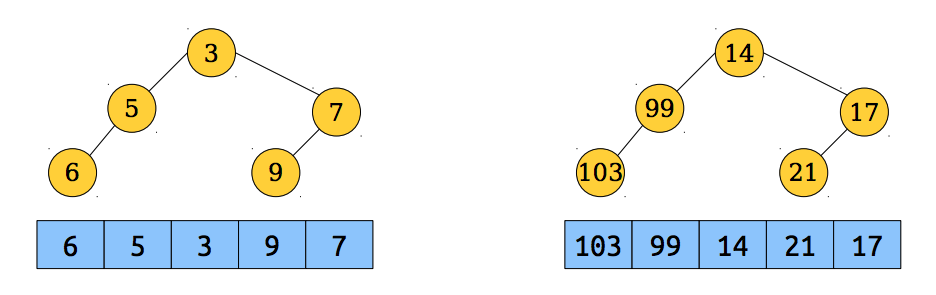
\includegraphics[scale=0.25]{cartesian}
\caption{Cartesian trees}
\end{figure}

A \emphasis{Cartesian tree} is defined as a binary tree which has a root that stores the minimum value and
whose left and right children are Cartesian trees built from the subarrays to the left
and right of the minimum. An alternative definition is a binary tree where an inorder traversal yields the original array
and is a min-heap.

We now have the following theorem: \( B_1 \sim B_2 \) iff \( B_1 \) and \( B_2 \)
have isomorphic, i.e. same shape Cartesian trees. Let's prove the forward direction
(\( B_1 \sim B_2 \implies \text{isomorphic Cartesian trees}\)): since \( B_1 \) and \( B_2 \)
have minima in the same positions as all RMQ queries are the same, their Cartesian trees must have
the same shape. To prove the reverse direction (\( \text{isomorphic Cartesian trees} \implies B_1 \sim B_2 \)),
notice that RMQ queries can be answered with an inorder traversal of a Cartesian tree.
Starting at the root, maintain a smallest element, start updating that element when you first see the
left index \( i \), and stop updating when you see the right index \( j \). A node is smaller if it is higher up
in the tree, i.e. it has a lower height. \\
Since we proved an ``if and only if'', the two conditions
are identical and thus there does not exist a ``tighter'' condition.

In order to check whether two arrays have isomorphic Cartesian trees, we need to be able to
build a Cartesian tree quickly. The algorithm is going to be inductive -
given a Cartesian tree built from \( n - 1 \) elements, we're going to extend it to \( n \).
A Cartesian tree for one element is just simply one node.
In order to maintain the fact that an inorder traversal yields the original array,
new nodes must be added as right children with the previous elements to their left.
In order to maintain the fact that the tree is a min-heap,
we can only add a new node as a child of nodes it's greater than.

These two observations form the following algorithm:
\begin{itemize}
  \item Keep a stack of ``active'' nodes.
  \item To insert a new node:
    \begin{itemize}
      \item While the stack is not empty and the top node has a value greater than the new node:
      \begin{itemize}
        \item Pop nodes off the stack
      \end{itemize}
      \item Make the parent of the new node the top of the stack, or null
      if the stack is empty (the new node is now the root).
      \item Make the left child of the new node the last node that was popped off the stack,
      null if nothing was popped off.
      \item Add the new node to the stack.
    \end{itemize}
\end{itemize}

Although this algorithm has a nested loop, each node is visted at most twice:
once on entering the stack and once when popped off. Therefore, this algorithm
runs in \( \Theta(n) \) and does at most \( 2n \) operations.

In order to check whether two trees are isomorphic, we can use a shortcut.
Instead of actually generating the Cartesian tree for a particular array, notice that
the resulting Cartesian tree is determined by the sequence of pushes and pops from the stack.
If we call a push ``1'' and a pop ``0'', then we have a binary number we'll call the
\emphasis{Cartesian tree number} with length at most \( 2n \). In order to compare two arrays,
we'll compare the two Cartesian tree numbers (padding with extra 0's if the length is less than \( 2n \)).
This approach answers our first question of determining whether \( B_1 \sim B_2 \), but
we still need to determine how many possible unique blocks there are. If our number is at most \( 2b \) bits long,
where \( b \) is the size of each block, then there are at most \(2^{2b} = 4^b \) possible numbers
(the actual number is determined by \href{https://en.wikipedia.org/wiki/Catalan_number}{Catalan numbers}
and is equal to \( \frac{1}{b + 1} \binom{2b}{b} \approx \frac{4^b}{b^{3/2}\sqrt{\pi}}) \).

\newpage

\subsection{The Final Algorithm}

\begin{figure}[h]
\centering
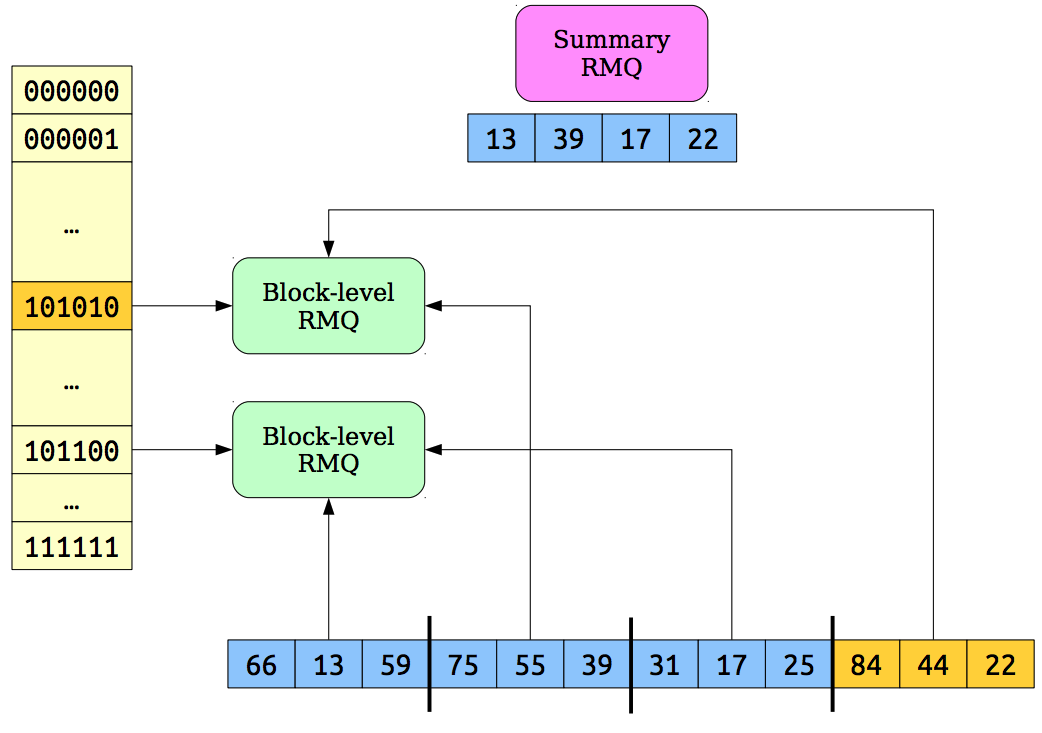
\includegraphics[scale=0.25]{final}
\caption{The final RMQ structure}
\end{figure}

Recall that we used a sparse table on the summary array with full precomputation on each block,
yielding a query time of \( O(1) \). Our precomputation time is:
\[ O(n + \frac{n}{b} \log n + (\text{\# of distinct blocks}) b^2) \]
and with our Cartesian tree observation, the number of distinct blocks is at most \( 4^b \).
\[ O(n + \frac{n}{b} \log n + 4^b b^2) \]
In order to pick \( b \), note that \( 4^b \) grows exponentially if \( b > \log n \), and \( \frac{n}{b} \log n \)
will be greater than \( n \) if \( b < \log n \). Thus, we should pick \( b = k \log_4 n \) where \( k \) is some constant.
\[ O(n + \frac{n}{k \log_4 n} \log n + 4^{k \log_4 n} (k \log_4 n)^2) \]
\[ O(n + n + n^k (k \log_4 n)^2) \]
In order to analyze the last term, we'll have to go on a mathematical tangent.

A function \( f(n) \) is \emphasis{polylogarithmically bounded} if \( f(n) = O( \log^k n) \)
for some constant \( k \).

Theorem: Any positive polynomial function grows faster than any polylogarithmic function,
i.e. \( \log^b n = o(n^a) \) for any constants \( a, b > 0 \).

Lemma: \( \lim_{x \to \infty} x^k = \infty \; \forall k \geq 0 \).
Proof: let \( c \) be some constant.
\[ x^k \geq c \]
\[ x \geq c^{\frac{1}{k}} \]
Since \( c^{\frac{1}{k}} \) is constant, for any constant \( c \), \( x^k \) can
exceed it if \( x \) is big enough, thus the limit is equal to infinity.

A direct proof of the theorem is to setup an infinite limit from the definition of \( o \):
\[ \lim_{x \to \infty} \frac{(\log x)^{b}}{x^a} \]
Use L'Hôpital's rule to evaluate the indeterminate form
\[ = \lim_{x \to \infty} \frac{b (\log x)^{b - 1} \cdot \frac{1}{x}}{a x^{a - 1}} \]
\[ = \lim_{x \to \infty} \frac{b}{a} \frac{(\log x)^{b - 1}}{x^a} \]
This results in another indeterminate form. Repeat taking derivatives until the power \( \log x \) is raised to
is less than 0, showing the limit is equal to 0 as the denominator approaches infinity.

A more intuitive proof results from the fact that exponents grow faster than polynomials,
i.e. \( n^b = o(a^n) \; \forall a > 1\).
\[ \lim_{x \to \infty} \frac{x^b}{a^x} \]
\[ = \lim_{x \to \infty} \frac{bx^{b - 1}}{(\ln a) a^x} \]
Repeat taking derivatives until the power \( x \) is raised to is less than 0,
showing the limit is equal to 0 as the denominator approaches infinity.

Substitute \( n = \log x \), resulting in \( (\log x)^b = o(a^{\log x}) \)
which is equivalent to \( o(x^{\frac{1}{\log a}}) \) by change of base, and
thus \( \log^b n = o(n^a) \).

Going back to the expression we had for the preprocessing time:
\[ O(n + n + n^k (k \log_4 n)^2) \]

In order to make this linear, \( k < 1 \), or else \( n^k \) will not be linear,
and \( k > 0 \) since block size can't be 0. Thus, we can pick any value in
\( 0 < k < 1 \) and essentially ignore the \( (\log n)^2 \) term since it is bounded
by any polynomial. The standard pick is \( k = \frac{1}{2} \), but that seems mostly arbitrary.

To conclude, we now have a \emphasis{Fischer-Heun structure} that solves RMQ
in an asymptotically optimal \( \langle O(n), O(1) \rangle \).

\begin{itemize}
  \item Set \( b = k \log_4 n = \frac{1}{2} k \log_2 n \) where \( k = \frac{1}{2} \).
  \item Split the array into blocks of size \( b \) and calculate the minimum for each block.
  \item Build a sparse table on that minima array.
  \item Build fully preprocessed RMQ structures on each block, avoiding recomputing the
  same RMQ structure for blocks with the same Cartesian tree number.
  \item Answer queries using the standard hybrid approach.
\end{itemize}

A sample implementation can be found \href{https://gist.github.com/stephen-huan/aa609965c86d750736398c28b025f9be#range-minimum-query}{here}.

\section{Sample Problems}

\begin{enumerate}
  \item \href{https://www.spoj.com/problems/RMQSQ/}{SPOJ RMQSQ}: Direct application of RMQ.

  \item \href{http://www.usaco.org/index.php?page=viewproblem2&cpid=576}{USACO Max Flow}
  or any problem involving Lowest Common Ancestor (LCA).
  LCA can be converted into RMQ in linear time and vice versa - the method is to
  perform an Euler tour on the tree. An Euler tour is essentially a combination of a
  preorder traversal and a postorder traversal that yields a list of nodes.
  If a node has children, we add it to the list and then recursively
  DFS on its children. After the recursive DFS call, we add the node to the list again.
  The LCA between two nodes in the graph must appear between the two nodes in this array.
  Other nodes not on the path between the two nodes may also appear between them,
  but they are guaranteed to have greater heights than the LCA.

  Some implementation details: I maintain a dictionary mapping a node to its first
  occurence in the array, the array itself, which contains the height of each node,
  and an inverse array mapping a position in the array to the node which it represents. \\
  The LCA between two nodes \( u, v \) is then inverse[RMQ(array, indexes[u], indexes[v])].

  \item \href{https://www.spoj.com/problems/BEADS/}{SPOJ BEADS}, \href{https://www.spoj.com/problems/LPS/}{SPOJ LPS},
  \href{https://leetcode.com/problems/longest-palindromic-substring/}{Leetcode LPS}, \href{https://leetcode.com/problems/palindromic-substrings/}{Leetcode palindromic-substrings}, etc.

  The \emphasis{L}ongest \emphasis{C}ommon \emphasis{P}refix (LCP) is
  the length of the longest common prefix between two strings.
  For example, the LCP between ``abcd'' and ``abef'' is 2.
  The \emphasis{LCP array} is then the LCP value between adjacent suffixes in the suffix array
  (the suffix array stores all of the suffixes of a given string sorted lexicographically).

  However, our LCP array only stores the LCP value for adjacent suffixes.
  How do we generalize to the LCP between any two suffixes?

  The observation is that the LCP value between two nonadjacent suffixes
  is the minimum LCP value between them in the LCP array.
  To see why this is true, notice that LCP decreases monotonically moving away from a suffix.
  Since the suffix array is sorted lexicographically, suffixes with a larger LCP
  value must be closer than suffixes with a smaller LCP value to a particular suffix.
  Call the LCP value \( h \) and the minimum LCP value between the two suffixes \( m \).
  \( h \leq m \) because of monotonicity.
  Also, \( h \geq m \) because a range minimum of \( m \) implies that there exists a prefix of length \( m \)
  common to all the suffixes between two suffixes, thus the LCP is at least \( m \).
  If \( m \leq h \leq m \), then \( h = m \).

  Thus, we can construct the Fischer-Heun RMQ structure on the LCP array.
  Then, the LCP between two suffixes \( i \) and \( j \) is lcp[rmq(lcp, i, j - 1)] assuming \( i \leq j \)
  which is an \( O(1) \) query. This allows us to solve a variety of string problems.

  \item RMQ can simulate a sliding window/monotonic queue.

\end{enumerate}

\newpage

\section{Picking \( k \)}

Why don't we use derivatives to optimize \( b \) like before?
Try solving
\[ -\frac{n \ln(\frac{n}{b})}{b^2 \ln 2} - \frac{n}{b^2 \ln 2} +
4^b b^2 \ln 4 + 2b 4^b = 0 \]
with no assumptions about \( b \).
Or, assuming \( b = k \log_4 n \):
\[ \frac{k^2 n^k \ln^3 n}{\ln^2 4} + \frac{2k n^k \ln^2 n}{\ln^2 4}
- \frac{n \ln 4 \ln{\frac{n \ln 4}{k \ln n}}}{k^2 \ln 2 \ln n}
- \frac{n \ln 4}{k^2 \ln 2 \ln n} = 0 \]
These equations may not be mathematically solvable.

As previously mentioned, \( k \) is empirically determined. My \( 2^n \) jump pointer solution
on USACO Max Flow (aforementioned) gets 12/15 of the testcases. Fischer-Heun, however,
gets 8/15 with \( k = \frac{1}{2} \). At this point, the reader may be tempted to exclaim ``I told you so!''.
With any complex algorithm, there is always the temptation to say ``While asymptotically optimal,
the large constant factors make a tighter, asymptotically inferior algorithm outperform it in practice.''
Not in this case! With \( k = 1 \), Fischer-Heun achieves 15/15 on Max Flow. Thus, the choice of \( k \) is nontrivial.

On SPOJ RMQSQ, there are also modest performance gains: 1.39 seconds for \( k = \frac{1}{2} \)
compared to 0.98 seconds for \( k = 1 \).

\begin{figure}[h!]
    \centering
    \begin{subfigure}[b]{0.4 \textwidth}
        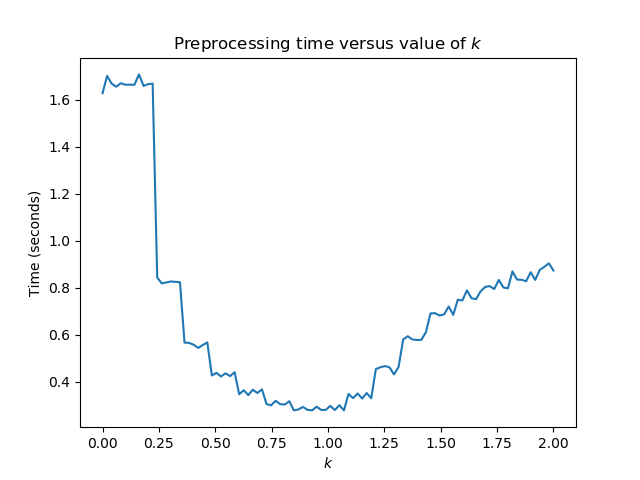
\includegraphics[width=1.5\textwidth]{preprocessing}
        \caption{Preprocessing time}
    \end{subfigure}
    \hfill
    \begin{subfigure}[b]{0.4 \textwidth}
        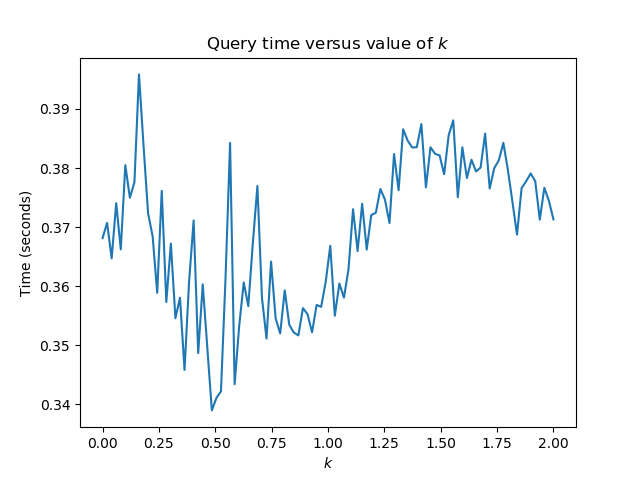
\includegraphics[width=1.5\textwidth]{query}
        \caption{Query time}
    \end{subfigure}
    \caption{Running time of the algorithm with varying \( k \)}
\end{figure}

The query times are basically random noise - the range is within 5 hundredths of a second.
This is to be expected as query is \( O(1) \) and independent of \( k \).

However, \( k \) does matter for preprocessing time, and the clear winner is \( k = 1 \).
This, coincidentally, is also probably the simplest choice.

\newpage

\section{Past Lectures}

\begin{enumerate}
  \item BITs
    \begin{enumerate}
      \item \href{https://activities.tjhsst.edu/sct/lectures/1920/2019_11_01_Binary_Index_Trees.pdf}{``Binary Indexed Trees'' (Patrick Zhang, 2019)}
      \item \href{https://activities.tjhsst.edu/sct/lectures/1819/2018_11_30_Binary_Indexed_Trees.pdf}{``Binary Indexed Trees'' (Daniel Wisdom, 2018)}
      \item \href{https://activities.tjhsst.edu/sct/lectures/1718/2017-11-10_Binary_Indexed_Trees.pdf}{``Binary Indexed Trees'' (Justin Zhang, 2017)}
      \item \href{https://activities.tjhsst.edu/sct/lectures/1213/bit_09_28_12.pdf}{``Binary Indexed Trees'' (Nick Haliday and Ryan Jian, 2012)}
    \end{enumerate}

  \item Segment trees
    \begin{enumerate}
      \item \href{https://activities.tjhsst.edu/sct/lectures/1920/2019_11_15_Segment_Trees.pdf}{``Segment Trees'' (Richard Zhan, 2019)}
      \item \href{https://activities.tjhsst.edu/sct/lectures/1819/2018_10_19_Segment_Trees.pdf}{``2018-10-19 Segment Trees'' (George Tang, 2018)}
      \item \href{https://activities.tjhsst.edu/sct/lectures/1718/2017-12-08_Segment_Trees.pdf}{``Segment Trees'' (Justin Zhang, 2017)}
      \item \href{https://activities.tjhsst.edu/sct/lectures/1617/2017-01-13_More_Segment_Trees.pdf}{``More Segment Trees'' (Kevin Geng, 2017)}
      \item \href{https://activities.tjhsst.edu/sct/lectures/1617/2016-10-28_Segment_Trees.pdf}{``Segment Trees'' (Charles Zhao, 2016)}
      \item \href{https://activities.tjhsst.edu/sct/lectures/1516/SCT_Segment_Tree.pdf}{``\( \sqrt{n} \) Bucketing and Segment Tree'' (Samuel Hsiang, 2015)}
      \item (Unavailable) ``Segment Tree (and its variants)'' \\ (Wassim Omais and Shwetark Patel, 2016)
    \end{enumerate}

  \item Lowest Common Ancestor
    \begin{enumerate}
       \item \href{https://activities.tjhsst.edu/sct/lectures/1920/2019_10_25_LCA.pdf}{``Lowest Common Ancestor'' (Richard Zhan, 2019)}
       \item \href{https://activities.tjhsst.edu/sct/lectures/1718/2017-12-01_Lowest_Common_Ancestor.pdf}{``Lowest Common Ancestor'' (Daniel Wisdom, 2017)}
       \item \href{https://activities.tjhsst.edu/sct/lectures/1617/2016-10-21_LCA_and_2_n_Jump_Pointers.pdf}{``LCA and \( 2^n \) Jump Pointers'' (Larry Wang, 2016)}
       \item \href{https://activities.tjhsst.edu/sct/lectures/1415/SCT_Lowest_Common_Ancestor.pdf}{``Lowest Common Ancestor'' [most similar to this lecture] \\ (Matthew Savage, 2015)}
    \end{enumerate}
  \item Longest Common Prefix
    \begin{enumerate}
      \item \href{https://activities.tjhsst.edu/sct/lectures/1819/2019_03_29_Suffix_Arrays_and_LCP.pdf}{``Suffix Arrays and Longest Common Prefix'' (Daniel Wisdom, 2019)}
      \item \href{http://web.stanford.edu/class/cs166/lectures/03/Slides03.pdf}{Constructing LCP array}
    \end{enumerate}
  \item \href{https://activities.tjhsst.edu/sct/lectures/1718/2018-02-09_USACO_Gold_Plat_January_Contest_Review_(square-root_decomposition).pdf}
  {``January Contest Review (\( \sqrt{N} \) decomposition'') \\ (Justin Zhang and Daniel Wisdom, 2018)}
  \item \href{https://activities.tjhsst.edu/sct/lectures/1718/2017-10-06_Simple_Range_Queries.pdf}{``Simple Range Queries'' (Justin Zhang, 2017)}
  \item \href{https://activities.tjhsst.edu/sct/lectures/1112/rquery102811.pdf}{``Advanced Data Structures'' [for RMQ] (Alex Chen, 2011)}
\end{enumerate}

\section{Works Cited}

\begin{enumerate}
  \item Stanford lectures
    \begin{enumerate}
      \item \href{http://web.stanford.edu/class/cs166/lectures/00/Slides00.pdf}{Part one}
      \item \href{http://web.stanford.edu/class/cs166/lectures/01/Slides01.pdf}{Part two}
    \end{enumerate}
\end{enumerate}

\end{document}
